% Chapter 1

\chapter{Introducción general} % Main chapter title

\label{Chapter1} % For referencing the chapter elsewhere, use \ref{Chapter1} 
\label{IntroGeneral}

%----------------------------------------------------------------------------------------

% Define some commands to keep the formatting separated from the content 
\newcommand{\keyword}[1]{\textbf{#1}}
\newcommand{\tabhead}[1]{\textbf{#1}}
\newcommand{\code}[1]{\texttt{#1}}
\newcommand{\file}[1]{\texttt{\bfseries#1}}
\newcommand{\option}[1]{\texttt{\itshape#1}}
\newcommand{\grados}{$^{\circ}$}

%----------------------------------------------------------------------------------------

En este capítulo se realiza una introducción al funcionamiento de un área de atención al cliente. Además, se menciona el estado del arte de los sistemas de procesamiento del lenguaje natural, y por último se explican los objetivos y alcances del presente trabajo.

%----------------------------------------------------------------------------------------
\section{Introducción}

En esta sección se introduce un área típica de atención al cliente en una empresa.

\subsection{Qué es la atención al cliente}

El área de atención al cliente se encarga de dar soporte al consumidor y tiene como objetivo resolver sus problemas \citep{WEBSITE:1}.

A menudo se confunde el área de atención con el área de servicio al cliente. La principal diferencia radica en que el servicio es una función proactiva con la intención de anticiparse a las necesidades inmediatas y a largo plazo del cliente. La atención al cliente es una función reactiva que busca resolver los problemas que el cliente manifestó \citep{WEBSITE:3}.

A continuación se listan las características principales del proceso \citep{WEBSITE:3}:
\begin{enumerate}

\item Inicio y duración: inicia cuando un cliente se pone en contacto con la empresa. Demora el tiempo que sea necesario hasta brindar una solución.
\item Objetivo: solucionar problemas que surjan del funcionamiento del producto o condiciones del servicio.
\item Actitud: reactiva.
\item Interacción: canales específicos. Por ejemplo, telefónicos, \textit{email} y \textit{chat}.
\item Participantes: cliente y representante del centro de atención. Raras veces entran en juego otros trabajadores de la empresa.

\end{enumerate}

\subsection{Organización de un equipo de atención al cliente}

A continuación se enumeran los principales roles que se pueden encontrar en el área de atención al cliente:

\begin{enumerate}

\item Gerente de atención al cliente: tiene bajo su responsabilidad el cumplimiento de metas estratégicas. Gestionan el volumen de casos entrantes y comunican las tendencias a otros departamentos. \citep{WEBSITE:6}
\item Coordinador de atención al cliente: es quien está en el día a día en contacto con los agentes. Apoya la resolución de problemas y escala aquellos que requieren validaciones o decisiones que no estén a su alcance \citep{WEBSITE:5}.
\item Analista de atención al cliente: canaliza las quejas, reclamos y sugerencias. Se encarga de proveer soporte a los usuarios. \citep{WEBSITE:5}

\end{enumerate}

En algunas organizaciones, dependiendo de su tamaño, se pueden encontrar más o menos mandos intermedios entre el gerente y el coordinador. Una variante puede ser tener varios coordinadores respondiendo a un supervisor. Este supervisor puede estar a cargo de la atención de reclamos para ciertos productos de la empresa que están relacionados.

En la figura \ref{fig:atencionestructura} se puede ver la principal tendencia que hay en cuanto a organización de equipos. La idea es que cada equipo sea especialista en un conjunto de casos.

\begin{figure}[htbp]
	\centering
	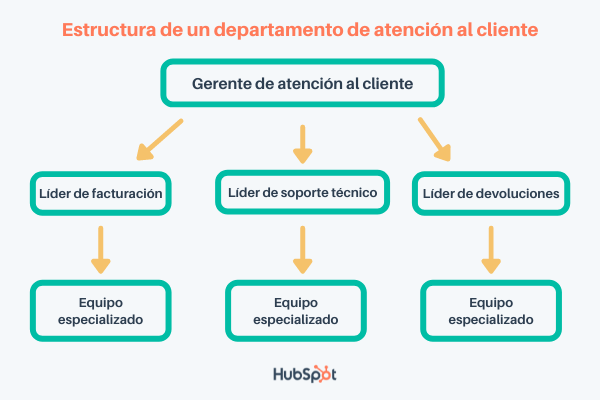
\includegraphics[width=.8\textwidth]{./Figures/atencionclienteestructura.png}
	\caption{Organigrama de un área de atención al cliente\protect\footnotemark.}
	\label{fig:atencionestructura}
\end{figure}

\footnotetext{Imagen tomada de \url{https://blog.hubspot.es/service/que-es-atencion-al-cliente}}

\subsection{El proceso de atención al cliente}

El proceso de atención al cliente consiste en una serie de pasos que se realizan para atender los reclamos y/o consultas que recibe la empresa \citep{WEBSITE:7}.

A continuación se describen los pasos principales de un proceso de atención típico \citep{WEBSITE:8}.

\begin{itemize}

\item Contacto y captura de la demanda del cliente: en esta etapa se recibe el mensaje del cliente por cualquiera de los canales establecidos y se procede a registrarlo en el sistema.
\item Análisis y clasificación: se analiza la información recibida y se evalúa si es suficiente para proceder a la clasificación del caso. De lo contrario se vuelve a contactar al cliente para obtener más detalles.
\item Resolución: en esta etapa se busca dar una respuesta a la consulta o reclamo del cliente. En algunos casos puede involucrar varios equipos o personas, por lo que su duración es variable.
\item Cierre: en esta etapa se presenta la solución al cliente y se le comunican los próximos pasos si los hubiera.

\end{itemize}

%----------------------------------------------------------------------------------------

\section{Motivación}

En la actualidad, resulta sumamente sencillo para el cliente optar por la competencia si la empresa no logra satisfacer sus expectativas. Una mala \textit{CX (Customer Experience)} puede generar un efecto de bola de nieve, ya que los usuarios que hayan tenido una mala experiencia, son mas propensos a comunicarlo con sus conocidos haciendo que la empresa no sólo pierda un cliente sino que además, se le dificulte expandir su mercado \citep{WEBSITE:9}.

Según informes de \textit{CX Trends} \citep{cxtrends}\citep{WEBSITE:4}\citep{WEBSITE:10} y de Esteban Kolsky \citep{WEBSITE:11}:

\begin{itemize}
\item El 70\% de los consumidores gastará más en una empresa que ofrezca una buena \textit{CX}.
\item El 50\% de los clientes se pasaría a la competencia después de haber tenido tan solo una mala experiencia. Este valor sube a un 80\% si se les pregunta si hubieran tenido dos o más malas experiencias.
\item El 72\% de los clientes compartiría una experiencia positiva con 6 o más personas.
\item El 13\% de los clientes compartiría su experiencia con 15 o más personas si no está satisfecho.
\item Sólo el 3,85\% de los clientes insatisfechos se lo comunican a la empresa.
\end{itemize}

Estos números muestran que la ausencia de quejas no es un signo de satisfacción. Por el contrario, es probable que los clientes hayan abandonado la empresa y estén compartiendo su insatisfacción con otras personas. También muestran la importancia de mantenerlos satisfechos, ya que son propensos a divulgarlo.

Más aún, entre las principales razones de una mala atención al cliente se encuentran tener tiempos de espera demasiado largos \citep{WEBSITE:12} y tener muchas derivaciones internas \citep{WEBSITE:13}.

De lo anterior se infiere que resulta muy importante que los procesos del área se realicen de forma eficiente. La utilización de modelos de IA para automatizar el proceso de clasificación de reclamos y consultas, ayuda a la empresa a responder a sus clientes con tiempos de respuesta menores y permite disponer de más analistas en la etapa de resolución y cierre. De esta manera, se genera una imagen positiva de la empresa que facilita la fidelización de clientes existentes y aumenta la incorporación de los nuevos.

%----------------------------------------------------------------------------------------

\section{Estado del arte}

El PNL (Procesamiento del lenguaje natural) es un subcampo de la inteligencia artificial que busca enseñar a un programa informático a comprender, interpretar y generar texto en lenguaje humano. A principios del siglo XXI, el PNL experimentó un crecimiento significativo gracias a la aplicación de algoritmos de aprendizaje profundo y la disponibilidad de grandes corpus de texto \citep{WEBSITE:14}.

\subsection{Word Embeddings}

En 2003 se entrena la primer red neuronal orientada al lenguaje utilizando vectores para representar palabras. Llamarían a este proceso ``aprender una representación distribuida para cada palabra'' \citep{ARTICLE:1}.

En 2008 se introduce el concepto de \textit{Word Embeddings} como una herramienta potente para tareas de PNL. Se distinguirían de sus antecesores mencionando que su objetivo era predecir la relevancia de una palabra dada la parte previa y posterior de la oración, a diferencia del trabajo previo que buscaba predecir la probabilidad de una palabra dada la parte previa de una oración.

En 2013, publican un artículo dónde detallan las arquitecturas \textit{CBOW} y \textit{Skip-Gram}. Además liberan el primer modelo pre-entrenado llamado \textit{Word2Vec} (basado en \textit{Skip-Gram}) popularizando el uso de los \textit{Word Embeddings} \citep{ARTICLE:3}.

Posteriormente, en 2014 publicarían \textit{GloVe} como otro método de generación de \textit{Word Embeddings} que utiliza una probabilidad de co-ocurrencia \citep{ARTICLE:4}. Con esta técnica, si dos palabras co-existen muchas veces, ambas palabras tienen una probabilidad alta de tener un mismo significado.

Los \textit{Word Embeddings} se convirtieron en la herramienta principal dentro del PNL. Capturan el significado de una palabra y la traducen a una representación numérica que puede ser usada como entrada para las redes neuronales.

\subsection{Transformers}

El avance del aprendizaje profundo, permitió a los investigadores desarrollar arquitecturas de redes neuronales más avanzadas y eficientes. 

Sin embargo, el verdadero hito no fue hasta 2017, cuando se publica la utilización de un mecanismo de atención para desarrollar una nueva arquitectura que se llamaría \textit{Transformers} \citep{ARTICLE:5}. Las redes más usadas hoy en día están basadas en esta mejora.

Básicamente, en los \textit{Transformers} se reemplazan las capas recurrentes que se venían utilizando hasta ese momento por ``capas de atención'' que codifican cada palabra en función del resto de la frase, permitiendo de esta forma, introducir el contexto en la representación matemática del texto. Por este motivo, sus \textit{Embeddings} generados son denominados \textit{Embeddings} contextuales.

Otra de las innovaciones introducidas es el uso de \textit{Embeddings} posicionales. Con ellos se logra una mayor paralelización, ya que no es más necesario pasar una palabra a la vez. Agregando un valor secuencial con cada palabra, hacen posible pasarle a la red todas las palabras en simultáneo.

Estas redes fueron evolucionando en tamaño y complejidad conforme transcurría el tiempo. En la figura \ref{fig:transformers} se puede ver la evolución de la cantidad de parámetros de estas redes a lo largo de los años.

\begin{figure}[htbp]
	\centering
	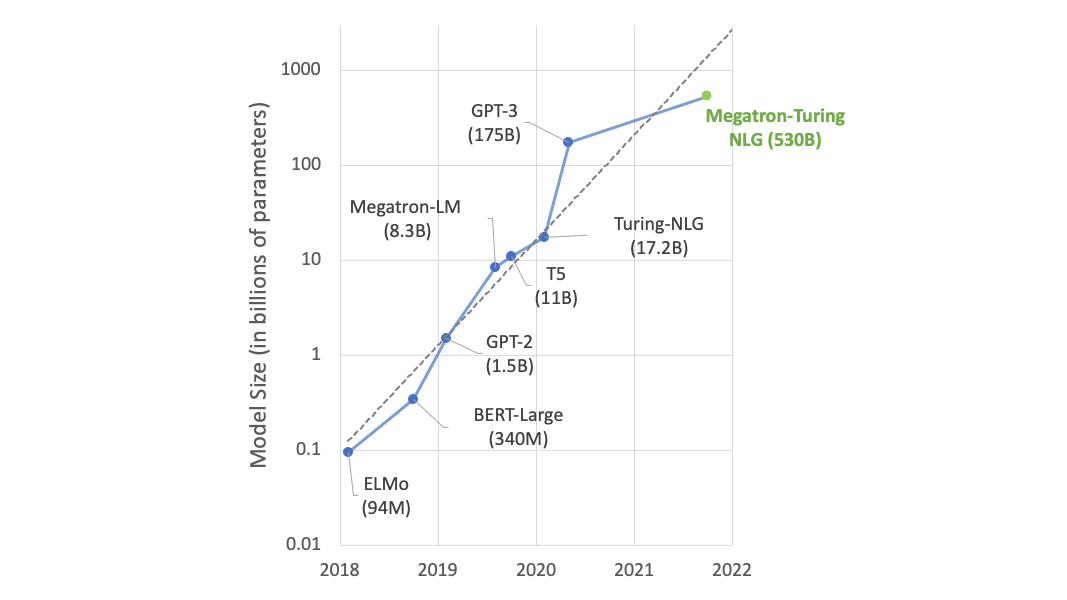
\includegraphics[width=1\textwidth]{./Figures/transformers.png}
	\caption{Evolución de las redes en cantidad de parámetros.\protect\footnotemark.}
	\label{fig:transformers}
\end{figure}

\footnotetext{Imagen tomada de \url{https://developer.nvidia.com/blog/using-deepspeed-and-megatron-to-train-megatron-turing-nlg-530b-the-worlds-largest-and-most-powerful-generative-language-model/}}

Los modelos basados en \textit{Transformers} se convirtieron en el modelo por defecto para tareas como traducción, clasificación de texto y resumen de textos, por citar algunos ejemplos.

En el área de atención al cliente, los principales usos de estas redes son \citep{WEBSITE:15}:
\begin{itemize}
\item \textit{Chatbots}: ayudan a responder consultas de forma inmediata evitando filas de espera.
\item Análisis de sentimiento: para realizar análisis sobre comentarios y quejas de los clientes.
\item Redireccionamiento de tickets: eliminan cuellos de botella en la parte de clasificación al redirigir el ticket directamente al área correspondiente.
\end{itemize}

%----------------------------------------------------------------------------------------

\section{Objetivos y alcance}

\subsection{Objetivos}

El propósito de este trabajo fue el desarrollo de modelos de inteligencia artificial (IA) para mejorar y agilizar la atención al cliente. Para lograr este objetivo es necesario realizar la clasificación automática de los reclamos de usuario en categorías de primer y segundo nivel.

En la figura \ref{fig:diag1} se presenta un diagrama de alto nivel de la solución. Se observa que en primera instancia, los reclamos se reciben por correo y chat, y luego son registrados en Salesforce, el sistema de CRM \textit{(Customer Relationsip Management)} que utiliza el área de atención al cliente \citep{WEBSITE:29}. Estos datos se replican en BigQuery a través de un proceso orquestado por Apache Airflow \citep{WEBSITE:30} \citep{WEBSITE:31}.

\begin{figure}[htbp]
	\centering
	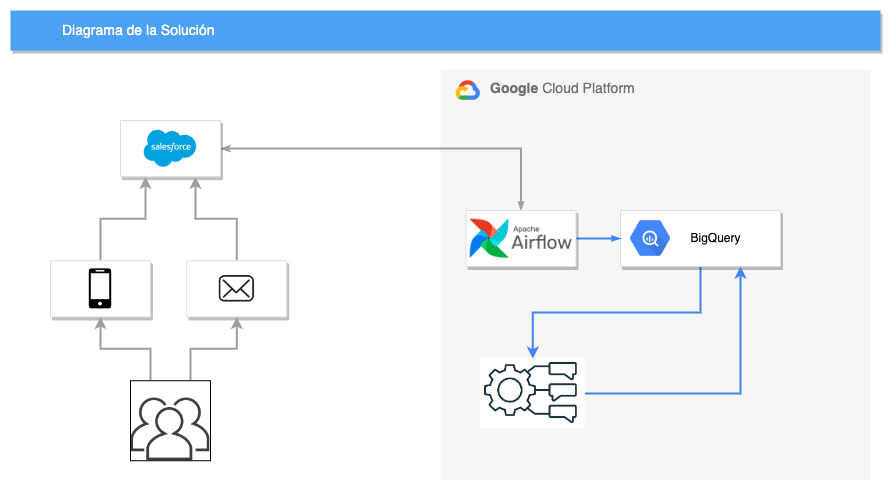
\includegraphics[width=.8\textwidth]{./Figures/solucion1.png}
	\caption{Diagrama general de la solución.}
	\label{fig:diag1}
\end{figure}

Los modelos de IA clasifican los casos que están en BigQuery y guardan la categoría de primer y segundo nivel en una tabla que luego el usuario podrá utilizar.

\subsection{Alcance}

El alcance de este proyecto estuvo orientado a desarrollar un prototipo de solución de software que incluyó las siguientes actividades:
\begin{itemize}
\item Obtención de los datos: se corresponde con el análisis de las fuentes de datos disponibles, tanto para entrenar los modelos de IA como para la parte de predicción de nuevos casos.
\item Análisis exploratorio de los datos: se corresponde con las actividades necesarias para generar nuevos \textit{insights}, que sirvieron para guiar el desarrollo de los modelos.
\item Modelado: se corresponde con la generación de variables a partir de los datos disponibles.
\item Entrenamiento: se corresponde con el entrenamiento de los modelos a partir de las variables obtenidas. También incluye la selección del mejor modelo para cada clasificación.
\item Despliegue: se corresponde con el diseño de la infraestructura para ejecutar los modelos de IA y su despliegue en un ambiente no productivo.
\item Documentación: se corresponde con los documentos de soporte que explican los procesos de modelado, entrenamiento y despliegue.
\end{itemize}

El alcance de este trabajo no cubre:
\begin{itemize}
\item La adaptación de los modelos a nuevas categorías inexistentes en los años 2021 y 2022.
\item El despliegue de los modelos en un ambiente productivo.
\item El soporte de la infraestructura desplegada en el ambiente no productivo.
\end{itemize}